%%%%%%%%%%%%%%%%%%%%%%%%%%%%%%%%%%%%%%%%%
% Simple Sectioned Essay Template
% LaTeX Template
%
% This template has been downloaded from:
% http://www.latextemplates.com
%
% Note:
% The \lipsum[#] commands throughout this template generate dummy text
% to fill the template out. These commands should all be removed when 
% writing essay content.
%
%%%%%%%%%%%%%%%%%%%%%%%%%%%%%%%%%%%%%%%%%

%----------------------------------------------------------------------------------------
%	PACKAGES AND OTHER DOCUMENT CONFIGURATIONS
%----------------------------------------------------------------------------------------

\documentclass[12pt]{article} % Default font size is 12pt, it can be changed here

\usepackage{geometry} % Required to change the page size to A4

\usepackage[utf8]{inputenc} % Use this package to enable the use of special norwegian characters (æ, æ, å)

\geometry{a4paper} % Set the page size to be A4 as opposed to the default US Letter

\usepackage{graphicx} % Required for including pictures

\usepackage{float} % Allows putting an [H] in \begin{figure} to specify the exact location of the figure
\usepackage{wrapfig} % Allows in-line images such as the example fish picture

\usepackage{cite}

\usepackage{url}

\usepackage{pdfpages}

\usepackage{supertabular} % Used for tables

\usepackage{tocbibind}

\usepackage[parfill]{parskip} % Newline without indent

\usepackage{lipsum} % Used for inserting dummy 'Lorem ipsum' text into the template

\usepackage{array}
\linespread{1.2} % Line spacing

%\setlength\parindent{0pt} % Uncomment to remove all indentation from paragraphs

\graphicspath{{./Graphics}} % Specifies the directory where pictures are stored

\setcounter{tocdepth}{5} %to make it appears in TOC
%\setcounter{secnumdepth}{5} %to make it numbered

\usepackage{multirow}
\usepackage{xcolor}
\usepackage{listings} % needed for the inclusion of source code

\usepackage{longtable}

\begin{document}
%----------------------------------------------------------------------------------------
%	TITLE PAGE
%----------------------------------------------------------------------------------------

\begin{titlepage}

\newcommand{\HRule}{\rule{\linewidth}{0.5mm}} % Defines a new command for the horizontal lines, change thickness here

\center % Center everything on the page

\textsc{\LARGE Høgskolen i Gjøvik}\\[0.5cm] % Name of your university/college

\includegraphics[width=90px, height=90px]{./Graphics/Hig-logo.png}\\[0.8cm] % Include a department/university logo - this will require the graphicx package 403x403px
\textsc{\Large Ethical hacking and penetration testing}\\[0.5cm] % Major heading such as course name
\textsc{\large Group Project}\\[0.5cm] % Minor heading such as course title

\HRule \\[0.4cm]
{ \huge \bfseries QP-testing}\\[0.4cm] % Title of your document
\HRule \\[1.5cm]

\begin{minipage}{0.44\textwidth}
\begin{flushleft} \large
%\emph{Authors:}\\
Victor \textsc{Rudolfsson} - 120912\\ % Your name
Tommy \textsc{B. Ingdal} - 120913\\ % Your name
Halvor \textsc{Thoresen} - 120915\\ % Your name
Anders \textsc{Lium} - 141598\\ % Your name
\end{flushleft}
\end{minipage}

\vfill % Fill rest of the page with empty lines
{\large \today}\\[3cm] % Date, change the \today to a set date if you want to be precise

\end{titlepage}

%----------------------------------------------------------------------------------------
%	TABLE OF CONTENTS
%----------------------------------------------------------------------------------------
\tableofcontents % Include a table of contents
\newpage % Begins the essay on a new page instead of on the same page as the table of contents 

%----------------------------------------------------------------------------------------
%	Executive Summary
%----------------------------------------------------------------------------------------
\section{Executive Summary}

EHAPT Group 3 has been given the task to conduct a penetration test against HiGs offline lab consisting of three VMWare images simulating three hosts in a lab network. At all times VMWare was set to “Host Only” network mode, to make sure no scanning or attacks by misfortune could be launched on other networks than the lab network.\\
The goal of this penetration test was to gather as much information as possible of the lab network, and if possible gain access to one or more of the hosts. To obtain this Group 3 used Kali Linux and similar penetration testing platforms along with tools like Discovery \& Probing, Enumeration, Password cracking, Vulnerability assessment in OpenVAS/Nessus and Penetration using Metasploit.\\
The report is based on the vulnerabilityassessment report template \cite{reporttemplate} and the SANS penetration testing report template \cite{sans}
\subsection{Result Summary} 
Using scanning, enumeration and vulnerability assessments, Group 3 were able to find the following information on the lab network worth checking further:
\begin{itemize}
	\item M1 runs an older version of Windows and is exposable for two known vulnerabilities of high criticality in the SMB version and the DNS Resolution.
	\item M2 runs OpenBSD 3.x or 4.x, and with a potential vulnerable OpenSSH v 5.6 running.
	\item M3 runs Linux 2.6.x, and with potential vulnerabilities for Lighttpd 1.4.26 and Telnet.
\end{itemize}
Using Wireshark for sniffing network traffic on the Linux host, Group 3 was able to see a Telnet connection going to an external IP address. Using a man-in-the-middle attack stealing the external IP with ARP poisoning, then using dsniff to listening on the Telnet connection, it became clear that the user “john” was sending his sudo password in clear text. Using this, Group 3 could log into the host using Telnet, change the password of the root user and escalate our privileges to root level.\\
With root access to M3, Group 3 was able to extract the password hashes containing user names and passwords for two other network users, “user” and “jane”. Using a password cracker, it was possible to guess the password of both these users in relatively short time, as the passwords consisted of plain text only. \\
Further, Group 3 discovered that the usernames and passwords from M3 were used on other hosts as well. With this, it was possible to log in with SAMBA “User” on M1 and with SSH “Jane” on M2 and thus obtaining access to all hosts in the lab network.\\
Although not exploited in this penetration test, several other vulnerabilities were found as well. \\
The Lighttpd 1.4.26 version running on M3 are vulnerable to SQL injection or Path traversal that this penetration tests documents could be utilized to cause Internal Server Error (possible DoS), and potentially also remote access shell although not documented here.\\
The OpenSSH version running on M2, along with the discovered login information, were further exploitable in terms of Group 3 being able to list out more information on users on this host and existing shares.\\
On the M1 host, the vulnerability related to DNS Resolution is known to be attackable using Denial-of-Service.\\
 % Includes the file that contains the introduction

%----------------------------------------------------------------------------------------
%	INTRODUCTION
%----------------------------------------------------------------------------------------
\section{Introduction}

\begin{longtable}{|p{16.5cm}|}
\hline
\textbf{Timeframe:} 15/10/14 - 04/11/14  \\ \hline
\textbf{Testing Team details }
\begin{itemize}
	\item Name: Victor Rudolfsson
	\begin{itemize}
		\item victor[.]rudolfsson[@]hig[.]no
		\item University college student
	\end{itemize}
	\item Name: Tommy B. Ingdal
	\begin{itemize}
		\item Tommy[.]ingdal[@]hig[.]no
		\item University college student
	\end{itemize}
	\item Name: Anders Lium
	\begin{itemize}
		\item Anders[.]lium[@]hig[.]no
		\item Telenor employee
	\end{itemize}
	\item Name: Halvor M. Thoresen
	\begin{itemize}
		\item Halvor[.]thoresen[@]hig[.]no
		\item University college student
	\end{itemize}
\end{itemize}
\\ \hline
\textbf{Network Details }
\begin{enumerate}
	\item \textbf{Host:} M1
		\begin{itemize}
			\item OS: Windows Vista Business (build 6000)
			\item IP: 192.168.248.131
		\end{itemize}
	\item \textbf{Host:} M2
		\begin{itemize}
			\item OS: OpenBSD
			\item IP: 192.168.248.130
		\end{itemize}
	\item \textbf{Host:} M3
		\begin{itemize}
			\item OS: Ubuntu 10.04.3
			\item IP: 192.168.248.132
		\end{itemize}
\end{enumerate}
\\ \hline
\textbf{Scope }
\begin{enumerate}
	\item \textbf{Constraints, limitations or problems}
		\begin{itemize}
			\item None
		\end{itemize}
	\item \textbf{Purpose of test}
		\begin{itemize}
			\item The penetration test was conducted to map out possible vulnerabilities and issues in the system. This is done to improve the overall security of the system.
		\end{itemize}
	\item \textbf{Type of test:}  Penetration test
	\item \textbf{Test type:} Black box
		\begin{itemize}
			\item The testing team had no knowledge of the network or computer setup prior to conducting the penetration test. 
		\end{itemize}
\end{enumerate}
\\ \hline
\end{longtable}  % Includes the file that contains the introduction

%----------------------------------------------------------------------------------------
%	Findingsl Summary
%----------------------------------------------------------------------------------------
\section{Summary of Findings}

This section will give a brief summary of the baseline security issues found and solutions to said issues, based on the technical findings. For how these security issues were ranked and categorized, refer to "Appendix F - Risk Calculations"
\begin{longtable}{|l|p{10.5cm}|} 

\hline
\multicolumn{2}{|l|}{\textbf{OS Security issues discovered}}                              \\ \hline
\multirow{2}{*}{\textbf{File System Security}} & Some users where found to have more privileges than they really needed.      \\ \cline{2-2} 
                                               & A policy on what the users should have access to should be implemented. \\ & Risk: Medium \\ \hline



\multirow{2}{*}{\textbf{Password Policy}} &  After compromising the stored hashed passwords, we found that the passwords generated weak hashes and could easily be cracked.    \\ \cline{2-2} 
                                               & A policy to use longer passwords and passphrases is strongly adviced. It is also recommended to enforce the policy on every system. This will make it harder to bruteforce or crack the hashed passwords in case of compromise. \\ & Risk: Medium \\ \hline



\multirow{2}{*}{\textbf{Patching Policy}} & All the machines in the network was running outdated operating systems.    \\ \cline{2-2} 
                                               & Operating systems should always be updated to the latest version to avoid critical vulnerabilities. \\ & Risk: Medium \\ \hline



\multirow{2}{*}{\textbf{Trust Policy}} & Some users with high privileges where found to have undesirable behavior which the penetration team were able to exploit.    \\ \cline{2-2} 
                                               & Even users with extensive IT knowledge should not be blindly trusting. It is recommended to regularly conduct a trust review to make sure users can be trusted with their privileges. \\ & Risk: High. \\ \hline


\multirow{2}{*}{\textbf{Trust Policy}} & Some users with high privileges where found to have undesirable behavior which the penetration team were able to exploit.    \\ \cline{2-2} 
                                               & Even users with extensive IT knowledge should not be blindly trusting. It is recommended to regularly conduct a trust review to make sure users can be trusted with their privileges. \\ & Risk: High. \\ \hline


\multirow{2}{*}{\textbf{Trust Policy}} & Some users with high privileges where found to have undesirable behavior which the penetration team were able to exploit.    \\ \cline{2-2} 
                                               & Even users with extensive IT knowledge should not be blindly trusting. It is recommended to regularly conduct a trust review to make sure users can be trusted with their privileges. \\ & Risk: High. \\ \hline

\end{longtable}


\begin{longtable}{|l|p{10.5cm}|} 
\hline
\multicolumn{2}{|l|}{Web Server Security}                              \\ \hline

\multirow{2}{*}{\textbf{Patching Policy}} & The version of the web server running was found to be vulnerable to multiple exploits. These include shellshock (CVE-2014-6271), SQLi exploitation and Path Traversal exploitation. These vulnerabilities can cause high impact.    \\ \cline{2-2} 
                                               & The web server is highly accessible from the outside, which significantly increases the threat. All vulnerabilities should be patched as soon as a patch is available. It is also highly recommended that a IDPS is implemented to detect and prevent attackers from accessing the systems. \\ & Risk: High \\ \hline

\end{longtable}

\newpage
Group 3 found that there are multiple highly critical issues as summarized in the table below.
\begin{table}[h]
\centering
\begin{tabular}{|l|l|l|}
\hline
Low & Medium & High \\ \hline
0   & 3      & 4    \\ \hline
\end{tabular}
\caption{Risk Table}
\end{table}

\begin{figure}[h!]
  \centering
    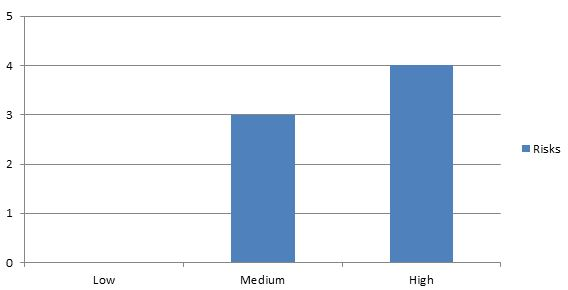
\includegraphics{./Graphics/riskchart.JPG}
 \caption{Risk compare chart.}
\end{figure}
 % Includes the file that contains the introduction

%----------------------------------------------------------------------------------------
%	Technical Summary
%----------------------------------------------------------------------------------------
\section{Technical Summary}

\begin{table}[h]
\begin{tabular}{|l|p{10.5cm}|} 
\hline
\multicolumn{2}{|l|}{OS Security issues discovered}                              \\ \hline
\multirow{2}{*}{\textbf{File System Security}} & Some users where found to have more privileges than they really needed.      \\ \cline{2-2} 
                                               & \textit{A policy on what the users should have access to should be implemented. \\ & Risk: Medium} \\ \hline



\multirow{2}{*}{\textbf{Password Policy}} &  After compromising the stored hashed passwords, we found that the passwords generated weak hashes and could easily be cracked.    \\ \cline{2-2} 
                                               & \textit{A policy to use longer passwords and passphrases is strongly adviced. It is also recommended to enforce the policy on every system. This will make it harder to bruteforce or crack the hashed passwords in case of compromise. \\ & Risk: Medium} \\ \hline



\multirow{2}{*}{\textbf{Patching Policy}} & \textit{All the machines in the network was running outdated operating systems.}    \\ \cline{2-2} 
                                               & \textit{Operating systems should always be updated to the latest version to avoid critical vulnerabilities \\ & Risk: Medium } \\ \hline



\multirow{2}{*}{\textbf{Trust Policy}} & \textit{Some users with high privileges where found to have undesirable behavior which the penetration team were able to exploit.}    \\ \cline{2-2} 
                                               & \textit{Even users with extensive IT knowledge should not be blindly trusting. It is recommended to regularly conduct a trust review to make sure users can be trusted with their privileges \\ & Risk: High.} \\ \hline

\end{tabular}
\end{table}

\begin{table}
\begin{tabular}{|l|p{10.5cm}|} 
\hline
\multicolumn{2}{|l|}{Web Server Security}                              \\ \hline

\multirow{2}{*}{\textbf{Patching Policy}} & \textit{The version of the web server running was found to be vulnerable to multiple exploits. These include shellshock (CVE-2014-6271), SQLi exploitation and Path Traversal exploitation. These vulnerabilities can cause high impact.}    \\ \cline{2-2} 
                                               & \textit{The web server is highly accessible from the outside, which significantly increases the threat. All vulnerabilities should be patched as soon as a patch is available. \\ & Risk: High} \\ \hline

\end{tabular}
\end{table} % Includes the file that contains the introduction

%----------------------------------------------------------------------------------------
%	Appendix A - Topology
%----------------------------------------------------------------------------------------
\include{AppA-Topology} % Includes the file that contains the introduction

%----------------------------------------------------------------------------------------
%	Appendix B - Definitions
%----------------------------------------------------------------------------------------
\section{Appendix B - Vulnerability Definitions} % Includes the file that contains the introduction

%----------------------------------------------------------------------------------------
%	Appendix C - Tools
%----------------------------------------------------------------------------------------
\section{Appendix C - Tools Utilised}

    \subsection*{Nessus}
    Nessus is a vulnerability scanner developed by Tenable Network Security. Today Nessus is on of the most used vulnerability scanners used in the pentesting field, alongside OpenVAS and CoreImpact.\\
    In this penetration test, Nessus was used in the start of the project in order to discover vulnerable services and servers in the network.
     
    \subsection*{OpenVAS}
    OpenVAS is a framework containing several services and tools related to vulnerability scanning. OpenVAS is open-source and free, making this product very popular amongst penetration testers worldwide.
     
    \subsection*{Metasploit}
    Metasploit is a very popular, open-source, framework created by Rapid7. Metasploit Framework is a tool for developing and executing exploits against vulnerable services/hosts, and contains thousands of different exploits, targeting Windows, Linux, BSD etc.
     
    \subsection*{Hashcat}
    Hashcat is a free password cracker with multi-gpu support. The authors claim that hashcat is the worlds fastest password cracker.\\
    We used hashcat when cracking the password we found during our assessment of the network.
     
    \subsection*{HashID}
    Hashid is a tool used to identify hashes. We used this tool to identify the hashes we found during the penetration test, in order to crack and recover the relevant passwords.
     
    \subsection*{NBTScan}
    NBTScan is a command line tool used to scan for NETBIOS nameservers on a network (local or remote). We used this tool in order to find open shares on the network.
     
    \subsection*{Dsniff}
    dsniff is a command line tool used to sniff passwords on a network. This tool handles everything from FTP and Telnet, to HTTP and RIP. This tool was used when we discovered the password transmitted over the Telnet protocol.
     
    \subsection*{Wireshark}
    This free and open-source packet analyzer is mainly used for network troubleshooting and network analysis. Wireshark can sniff and analyze about any protocol used to transfer data over a network, and this information can later be dumped and saved to a .pcap file for later analysis.\\
    This tool was used to sniff data going over the network and between the computers we did a penetration test on, in hope of finding anything that could be exploited.
     
    \subsection*{NMAP}
    NMAP (Network Mapper) is a network scanner used to discover hosts and services on a network, and thus create a map of the network. NMAP was used in conjunction with Wireshark to map out the entire network, and collect information about the hosts and services running on the network.
     
    \subsection*{Python}
    Python is a very poopular general-purpose programming language with a huge emphasis on code readability. We used this programming language to try out some exploits against the SMB protocol and a web server vulnerability.
     
    \subsection*{find}
    find is a built-in command in linux, used to find files.\\
    We used this command to find files with the setuid bit set, with the hope that one of those files could lead to command execution with root privileges.\\
   \vspace{-0.5cm}\begin{lstlisting}
find directory -user root -perm -4000 -exec ls -ldb {} \; >/tmp/filename
\end{lstlisting}

 % Includes the file that contains the introduction

%----------------------------------------------------------------------------------------
%	Appendix D - Scan results
%----------------------------------------------------------------------------------------
\section{Appendix D - Scan Results}

\definecolor{dkbrown}{RGB}{153, 51, 51}
\definecolor{dkgreen}{RGB}{0, 128, 0}

\lstset{
  language=java,
  numbers=left,
  numberstyle=\tiny\color{gray},
  stepnumber=1,
  numbersep=5pt,  
  backgroundcolor=\color{white},  % choose the background color. You must add \usepackage{color}
  showspaces=false,               % show spaces adding particular underscores
  showstringspaces=false,         % underline spaces within strings
  showtabs=false,                 % show tabs within strings adding particular underscores
  frame=single,                   % adds a frame around the code
  rulecolor=\color{black},        % if not set, the frame-color may be changed on line-breaks within not-black text (e.g. commens (green here))
  tabsize=4,                      % sets default tabsize to 2 spaces
  captionpos=b,                   % sets the caption-position to bottom
  breaklines=true,                % sets automatic line breaking
  breakatwhitespace=false,        % sets if automatic breaks should only happen at whitespace
  title=\lstname,
  linewidth=17.5cm, 
  basicstyle=\fontsize{8}{11}\ttfamily,
  xleftmargin=-2.75cm,
  keywordstyle=\color{blue},
  alsoletter={:~$},
  keywordstyle=\color{blue},
  commentstyle=\itshape\color{red},
  identifierstyle=\color{dkbrown},
  stringstyle=\color{orange},
}

\lstset{literate=%
{æ}{{\ae}}1
{å}{{\aa}}1
{ø}{{\o}}1
{Æ}{{\AE}}1
{Å}{{\AA}}1
{Ø}{{\O}}1
{\$}{{\textcolor{red}{\$}}}1 
         {:}{{\textcolor{red}{:}}}1
         {~}{{\textcolor{red}{\textasciitilde}}}1
}
\lstset{extendedchars=\true}
\lstset{inputencoding=ansinew}

\begin{lstlisting}[language=bash]
root:$6$x9LyUphj$3cQTGIb269GBNuKc6GER29W9Ht7NmHjMRlyeR35oTTqngQHVD4gupwzSmjhAYOc6KEyfGQ32De27SgOCNzKcE.:16371:0:99999:7:::

...

jane:$1$a0rCbP9/$1FKr5sobP4rQHxuTA/l/p.:16346:0:99999:7:::
telnetd:*:16346:0:99999:7:::
john:$6$4xE5VNT4$Vb0nrZ64DGZvWmEy9sUKkCaS9O5lb50WlzSIxim6ydaCVfzWJrmLuwZIPxjgw1ZDIeQB9C9jX7qb7AtiDibjo0:16346:0:99999:7:::
user:$6$Jp01V0lm$RX7eMjNIIoCnazLNEtSAe5Uq.nQINXMOpEggvRtTEV63QEMUEpmwFMJhYzQtLT/M33Kbl5Mhr59tPJbvN/u4k1:16346:0:99999:7:::
\end{lstlisting}

\begin{lstlisting}
root:$6$x9LyUphj$3cQTGIb269GBNuKc6GER29W9Ht7NmHjMRlyeR35oTTqngQHVD4gupwzSmjhAYOc6KEyfGQ32De27SgOCNzKcE.:16371:0:99999:7:::

...

jane:$1$a0rCbP9/$1FKr5sobP4rQHxuTA/l/p.:16346:0:99999:7:::
telnetd:*:16346:0:99999:7:::
john:$6$4xE5VNT4$Vb0nrZ64DGZvWmEy9sUKkCaS9O5lb50WlzSIxim6ydaCVfzWJrmLuwZIPxjgw1ZDIeQB9C9jX7qb7AtiDibjo0:16346:0:99999:7:::
user:$6$Jp01V0lm$RX7eMjNIIoCnazLNEtSAe5Uq.nQINXMOpEggvRtTEV63QEMUEpmwFMJhYzQtLT/M33Kbl5Mhr59tPJbvN/u4k1:16346:0:99999:7:::
\end{lstlisting} % Includes the file that contains the introduction

%----------------------------------------------------------------------------------------
%	Appendix E - Methods
%----------------------------------------------------------------------------------------
\section{Appendix C - Mothodology Utilised}

\begin{figure}[h!]
\centering
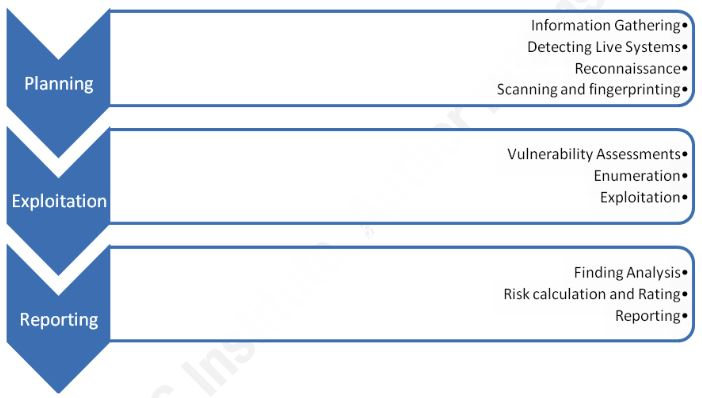
\includegraphics[scale=0.8]{./Graphics/sansmeth.JPG}
\caption{SANS methodology \cite{sans}}
\end{figure}

The penetration test was conducted by following the method described in the SANS penetration testing template \cite{sans}. \\
Exeptions are the information gathering and the reconnaissance phase. % Includes the file that contains the introduction

%----------------------------------------------------------------------------------------
%	Appendix F - Risk Calculations
%----------------------------------------------------------------------------------------
\section{Appendix D - Risk Calculations}

In order to categorize the vulnerabilites that are found, we have to define the categorizing measure. \\
In the penetration test has catogorized the vulnerabilites by risk. \\
The risk is calculated by multiplying the impact (damage done) and Threat (chance of impact). \(Risk = Imapct * Threat\) \\
\begin{table}[h]
\centering
\begin{tabular}{llllll}
\multirow{6}{*}{Threat} & \multicolumn{5}{c}{Impact}                                                                                                                                             \\ \cline{3-6} 
                        & \multicolumn{1}{l|}{}             & \multicolumn{1}{l|}{Low (1)} & \multicolumn{1}{l|}{Medium (2)} & \multicolumn{1}{l|}{High (3)} & \multicolumn{1}{l|}{Critical (4)} \\ \cline{2-6} 
                        & \multicolumn{1}{l|}{Low (1)}      & \multicolumn{1}{l|}{1}       & \multicolumn{1}{l|}{2}          & \multicolumn{1}{l|}{3}        & \multicolumn{1}{l|}{4}            \\ \cline{2-6} 
                        & \multicolumn{1}{l|}{Medium (2)}   & \multicolumn{1}{l|}{2}       & \multicolumn{1}{l|}{4}          & \multicolumn{1}{l|}{6}        & \multicolumn{1}{l|}{8}            \\ \cline{2-6} 
                        & \multicolumn{1}{l|}{High (3)}     & \multicolumn{1}{l|}{3}       & \multicolumn{1}{l|}{6}          & \multicolumn{1}{l|}{9}        & \multicolumn{1}{l|}{12}           \\ \cline{2-6} 
                        & \multicolumn{1}{l|}{Critical (4)} & \multicolumn{1}{l|}{4}       & \multicolumn{1}{l|}{8}          & \multicolumn{1}{l|}{12}       & \multicolumn{1}{l|}{16}           \\ \cline{2-6} 
\end{tabular}
\caption{Risk Table}
\label{my-label}
\end{table}

For the risk score to be used practically, we have to compress them into smaller categories as seen in table 2.

\begin{table}[h]
\centering
\begin{tabular}{|l|l|l|}
\hline
Low & Medium & High \\ \hline
1-4 & 5-8    & 9-16 \\ \hline
\end{tabular}
\caption{Risk categorization}
\label{my-label}
\end{table}
 % Includes the file that contains the introduction


%----------------------------------------------------------------------------------------
%	BIBLIOGRAPHY (References)
%----------------------------------------------------------------------------------------
\bibliographystyle{unsrt}
\bibliography{Sources}
%\begin{thebibliography}{99} % Bibliography - this is intentionally simple in this template

%\bibitem[Figueredo and Wolf, 2009]{Figueredo:2009dg}
%Figueredo, A.~J. and Wolf, P. S.~A. (2009).
%\newblock Assortative pairing and life history strategy - a cross-cultural
%  study.
%\newblock {\em Human Nature}, 20:317--330.
 
%\end{thebibliography}

%----------------------------------------------------------------------------------------------------------------------------------------------------
\end{document}